%% Version 6.1, 1 September 2021
%
%%%%%%%%%%%%%%%%%%%%%%%%%%%%%%%%%%%%%%%%%%%%%%%%%%%%%%%%%%%%%%%%%%%%%%%%%%%%%%%%%%%%%%%%%%%%%%%%%%%%%%%%%%%%%%%%%%%%%%%%%%%%%%%%%%%%%%%%%%%%%%%%%%%%%%%%%%%%%%%%%%%%%%%%%%%%%%%%%%%%%%%%%%%
% TemplateV6.1.tex --  LaTeX-based blank template for submissions to the 
% American Meteorological Society
%
% Start with one of the following:
% 1.5-SPACED VERSION FOR SUBMISSION TO THE AMS
% \documentclass{ametsocV6.1}

% TWO-COLUMN JOURNAL PAGE LAYOUT---FOR AUTHOR USE ONLY
% \documentclass[twocol]{ametsocV6.1}
\documentclass{ametsocV6.1}
\usepackage{xcolor}

%%%%%%%%%%%%%%%%%%%
% TITLE AND AUTHORS
\title{Bridging the scale gap: enhancing point-scale rainfall estimates by post-processing ERA5}

\authors{
Fatima M. Pillosu\aff{a,b}\correspondingauthor{Fatima Pillosu, tj835682@student.reading.ac.uk}
Timothy D. Hewson\aff{b}
Estibaliz Gascòn\aff{b}
Milana Vuckovic\aff{b}
Christel Prudhomme\aff{b,c,d}
Hannah Cloke\aff{a,e}
}

\affiliation{
\aff{a}{Department of Geography and Environmental Science, University of Reading, Reading, UK}\\
\aff{b}{Forecast and Services Department, European Centre for Medium-range Weather Forecasts, Reading, UK}\\
\aff{c}{Department of Geography and Environment, University of Loughborough, Loughborough, UK}\\
\aff{d}{UK Centre for Ecology and Hydrology, Wallingford, United Kingdom}\\
\aff{e}{Department of Meteorology, University of Reading, Reading, UK}\\
}

%%%%%%%%%%
% ABSTRACT
%%%%%%%%%%

\abstract{Accurately estimating rainfall distributions, from small to extreme totals, is crucial for addressing various environmental challenges, including flood forecasting, water resource management, and disaster preparedness. Global Numerical Weather Prediction (NWP) models can provide useful rainfall estimates; yet, they often misrepresent point-scale observations from rain gauges, underestimating the frequency of small rainfall totals and underestimating extreme values. This study provides a systematic, global verification of four NWP-modelled rainfall datasets with different resolutions - ERA5's Ensemble Data Assimilation (62 km, probabilistic), ERA5's short-range forecasts (31 km, deterministic), short-range ECMWF reforecasts for cycle 46r1 (18 km, control run), and ERA5-ecPoint (point-scale, probabilistic) - against 20 years of point-rainfall observations from rain gauges around the world. \textcolor{blue}{The analysis focuses on liquid precipitation and is not stratified by season, with observations pooled across all months to characterise the overall climatological distribution at each station.} The models' ability to represent the entire rainfall distribution, including extreme rainfall, was assessed. Overall, the higher spatial resolution of NWP models enables a more accurate representation of gauge-based climatologies. Nonetheless, ERA5-ecPoint provides the most accurate representation, capturing the frequency of zeros, the growth rates of rainfall totals, and the wet tails more accurately. Moreover, due to its probabilistic nature, ERA5-ecPoint can estimate long return periods (e.g., 1000 years and more), offering insights into extremely rare or unprecedented events at specific locations. The model significantly improves performance in flat, hilly/mountainous regions. In very mountainous areas (e.g., the Andes), it underestimates zero rainfall totals and overestimates the length of the wet tails. These findings underscore the importance of using post-processing to enhance the local-scale validity of global NWP models. Moreover, as climate change intensifies extreme rainfall events, these findings are crucial for estimating accurate long-period rainfall climatologies, as needed for effective mitigation and resilience building, particularly in areas lacking comprehensive and reliable rain gauge records.}


%%%%%%%%%%%%%%%%%%%%%%
% MAIN BODY OF PAPER %
%%%%%%%%%%%%%%%%%%%%%%

\begin{document}

\maketitle


%%%%%%%%%%%%%%%%%%%%%%%%
% Significance statement

SIGNIFICANCE STATEMENT: The purpose of this study is to better understand how modelled rainfall datasets represent the distribution of point-scale rainfall as measured by rain gauges, including extremes. We considered four modelled rainfall datasets, including ERA5 at 62 and 31 km, ECMWF reforecasts at 18 km, and the ecPoint post-processed version of ERA5 (ERA5-ecPoint), which produces probabilistic point-scale rainfall estimates. All models were evaluated against twenty years of rain gauge measurements worldwide. Our findings demonstrate that ERA5-ecPoint largely improves the estimates of point-rainfall, correctly capturing both small and extreme rainfall totals. This advancement is crucial since many regions lack (appropriate) rain gauge coverage. Moreover, as climate change intensifies extreme rainfall globally, ERA5-ecPoint enables planners to quantify rare, unseen events, providing crucial information for infrastructure design and disaster preparedness. 


%%%%%%%%%%%%%%%%%%%%%%
\section{Introduction}

Accurately estimating the full range of past and future rainfall distributions, from light to extreme totals, is one of the biggest challenges in modern meteorology. Yet, it is essential to address a range of critical issues. In flood forecasting, accurately estimating the spatial distribution of small and extreme rainfall totals influences the catchment response to the rainfall event, impacting runoff generation and streamflow patterns \citep{Cuo2011, WangKarimi2022}. In water resource management, understanding the full rainfall distribution informs the management of reservoirs for flood control, power generation, and irrigation purposes \citep{Tie2023}. It also helps in agricultural applications such as crop selection and planting schedules \citep{Janmohammadi2023, Maurya2024}. It also supports urban planning by helping to design effective urban drainage systems and manage storm-water runoff \citep{Hossain2024, Laouacheria2019}. Analysing changes over time in the entire rainfall distribution provides insights into climate change impacts such as shifts in the frequency and intensity of extreme rainfall events \citep{Tye2022}, droughts' characteristics \citep{Haile2020}, biodiversity and ecosystems stability \citep{Lamprecht2021}, and food security \citep{Balasundram2023}. Extreme rainfall, in particular, has received significant attention in recent literature \citep{Gimeno2022, Schumacher2017} due to its catastrophic impacts for society, infrastructure, and the environment \citep{IPCC2023, WMO2024}. It not only reduces worldwide macroeconomic growth rates and slows global economic rise \citep{Liang2022}, but also can cause long-term anxiety and post-traumatic stress on affected communities, hindering recovery efforts \citep{Doocy2013}. With climate change expected to intensify both the frequency and severity of extreme rainfall, even in regions where average precipitation is decreasing \citep{Asadieh2015, Westra2014, Zittis2021}, understanding its past and anticipating future trends is crucial to inform disaster preparedness and response efforts. 

Precipitation time series can be obtained from various sources. Rain gauges are a primary source of ground truth. They provide highly accurate direct point-scale precipitation measurements when properly maintained and calibrated \citep{LanzaStagi2008}. In regions with dense networks, rain gauges offer a good spatial representation of localised extremes \citep{Haiden2016}. Moreover, stations have been operating for decades in some locations, providing high-quality long-term historical records for trend analysis \citep{Anand2020, Tadeyo2020}. Rain gauge coverage is notably spatially and temporally uneven, leaving many regions unmonitored \citep{Kidd2017}. In areas with complex topography or low-density networks, gauges may fail to represent the rainfall's spatial variability \citep{DiCurzio2022}. Inadequate rain gauge maintenance can also lead to data gaps or inaccuracies \citep{LanzaStagi2008}. \textcolor{blue}{Furthermore, systematic quality control of gauge records remains challenging, as automated screening procedures may not reliably detect all forms of measurement error, including timing errors, blocked funnels, or spurious accumulations \citep{Wang2023}.} Satellite- and radar-derived gridded datasets provide broader spatial and temporal coverage, particularly in ungauged regions \citep{Herold2017}. Their rainfall estimates may, however, differ from rain gauge measurements, especially extremes which might be severely underestimated and mislocated \citep{Ensor2008, Gupta2020, Satge2020}. Numerical Weather Prediction (NWP) models, such as reanalyses and reforecasts, offer spatially and temporally consistent precipitation datasets with global, multi-decadal coverage. Reanalyses, like ERA5 and its Ensemble Data Assimilation (EDA) component \citep{Hersbach2020} or NCEP/NCAR Reanalysis \citep{Hamill2022, Kalnay1996}, integrate historical weather observations with a state-of-the-art NWP model to produce high-resolution precipitation datasets. Reforecasts, such as NCEP's Global Ensemble Forecast System \citep{Guan2022} and ECMWF's Integrated Forecast System \citep{Richardson2014}, provide 20-30 years of retrospective forecasts generated with current operational NWP models. Reanalyses capture rainfall's spatial patterns and temporal trends \citep{Lavers2022} but tend to underestimate extreme precipitation due to their coarse resolution of about 50 or 30 km \citep{Alexandridis2023, Donat2016, Espinosa2024, GomisCebolla2023}\footnote{Note that the studies comparing both ERA5 and ERA5-Land against rain gauge observations are considered in this study only for their analysis of ERA5. These are somewhat flawed as ERA5-Land simply re-grids, without any statistical or dynamical downscaling, the precipitation in ERA5 onto ERA5-Land's grid \citep{MunozSabater2021}.}. Reforecasts also capture rainfall's spatial patterns and temporal trends, but still underestimate extreme precipitation even though their resolution is half, i.e. 18 km \citep{Hewson2024}\footnote{Although ECMWF reforecasts are now produced at a horizontal resolution of approximately 9 km, \cite{Hewson2024} demonstrated that the magnitude of precipitation extremes does not increase substantially when moving from the previous 18 km resolution to 9 km, suggesting limited added value at the tail of the distribution from this resolution increase alone.}. \textcolor{magenta}{A fundamental challenge therefore persists: NWP grid-box values represent areal averages, whereas rain gauges measure precipitation at a single point, creating a scale gap that must be bridged (\textit{bridging the scale gap}) before modelled and observed climatologies can be meaningfully compared or operationally combined.} Statistical post-processing methods can enhance the local-scale representation of rainfall \citep{Giorgos2024}, but their effectiveness commonly depends on the availability of high-quality observations, leading to a patchy geographical coverage of post-processed reanalysis/reforecasts \citep{Vannitsem2021}. The post-processing method proposed by \cite{HewsonPillosu2021}, called ecPoint, improves the local-scale representation of NWP model outputs globally, particularly for extremes, without requiring high-density observational networks, using a non-local calibration strategy. The ecPoint approach was applied to ERA5 for rainfall and temperature through the Highlander project \citep{Hewson2023, Bottazzi2024}. 

The primary aim of this study is to assess the fitness-for-purpose of the ERA5-ecPoint dataset by comparing its representation of point rainfall climatologies around the world against the rain gauge-based equivalent. A secondary goal is to evaluate the impact of spatial resolution on the representation of point rainfall climatologies from three additional datasets: ERA5's Ensemble Data Assimilation (EDA, 62 km \textcolor{blue}{effective grid spacing}), ERA5's short-range forecasts (31 km), and ECMWF 46r1 reforecasts (18 km). Two research questions are, therefore, examined. How do NWP models represent the overall distribution of point-rainfall observations (RQ1)? How do NWP models represent, in particular, extreme rainfall (RQ2)? 
\textcolor{magenta}{With a reliable post-processed climatology in hand, one could analyse extreme rainfall trends over long periods (+80 years), place observed or forecast extremes into a climatological context, and assess whether a predicted event has historical precedent or lies beyond the range of physically plausible magnitudes.} 

The study is organised as follows. Section 2 describes the rain gauge observations and the NWP models used in this study. Section 3 describes the methods adopted to answer the research questions. Section 4 presents the results from the objective verification and a case study, while Section 5 discusses them. Final remarks are drawn in Section 6.

%%%%%%%%%%%%%%
\section{Data}

\subsection{Point-scale rain gauge precipitation observations}
This study considered 24-hourly precipitation from surface synoptic observations (SYNOP) from the Global Telecommunication System (GTS) network and additional gauge data stored internally at ECMWF. SYNOP observations consist of standardised, historical and near-real-time meteorological reports that ensure data quality and format consistency across diverse regions. High-density national rain gauge networks (primarily from European countries and available internally at ECMWF) were also integrated into the analysis \citep{Haiden2016}. 

\begin{table*}[h!]
\centering
\caption{\textcolor{blue}{Characteristics (columns 1 to 5) of the observational rainfall dataset (row 1) and the considered NWP models (rows 2 to 5), as well as their derived climatologies (columns 6 to 8). \textcolor{magenta}{It is worth noting that the unavailable data for ERA5-EDA (row 2, column 6) is due to sporadic damage to the storage tapes on which the original data were archived (MARS archive). These losses occurred at irregular intervals with no systematic temporal or spatial pattern. There is therefore no reason to expect that the missing data would introduce bias into the derived rainfall climatology.}}}
\includegraphics[width=16cm]{Figures/01_Datasets_Description.jpg}
\label{fig:Datasets_Description}
\end{table*}

\textcolor{blue}{Rain gauge networks are subject to well-documented issues, such as gauge undercatch and localised siting effects \citep{Pollock_2018, Kochendorfer_2020}, that cannot be fully eliminated through post-hoc quality control. The rain gauge observations used in this study underwent a multi-step quality control procedure prior to analysis. Rainfall frequency distributions were visually inspected across multiple intensity ranges to identify anomalous features, including suspicious peaks at regular intervals (e.g., 300, 310, 320 mm) suggestive of encoding or data transmission errors, artificial clustering at round integer values (e.g., 100, 200, 300 mm), and physically implausible totals exceeding known world records (1825 mm/24h, La Réunion). Flagged values were cross-checked against nearby stations (akin to buddy checking) and compared against the independent CPC Global Unified Gauge-Based Analysis\footnote{https://psl.noaa.gov/data/gridded/data.cpc.globalprecip.html}, a gridded product at 50 km resolution (akin to background checking). The CPC dataset was deliberately selected rather than ERA5 to preserve the independence of the verification framework. Comparison with the CPC data involved applying a scaling factor to account for representativeness differences between the gridded product and point-scale observations. After a sensitivity analysis, the scale factor of 20 was selected to clean erroneous rainfall observations. The procedure successfully removed the majority of anomalous features whilst yielding distributions more consistent with expected climatological behavior. Notwithstanding these efforts, we acknowledge that some observational errors may remain undetected. However, the relative comparison between datasets is less sensitive to such biases, given the common observational reference used throughout.}

Rain gauge observations stored at ECMWF have increased considerably since the 2000s. Thus, we consider a 20-year verification period between the 1\textsuperscript{st} of January 2000 to the 31\textsuperscript{st} of December 2019. \textcolor{blue}{Since the verification in this study is conducted at the climatological level — comparing full distributions of 24-hourly accumulations rather than matching individual events on a timestep-by-timestep basis — the analysis was not restricted to a single accumulation window. For each station, 24-hourly rainfall climatologies were computed using the accumulation window consistent with the station's reporting time (e.g., 00–00, 01–01, 02–02 UTC, and so on). This approach maximises spatial coverage by retaining stations in regions where reporting times do not align with the 00 UTC convention, such as parts of South Asia and Australasia. The resulting station-level climatologies were then pooled into a single verification database. This aggregation is considered defensible because, over a 20-year record, the statistical distribution of 24-hourly totals at a given location is not expected to vary substantially with modest shifts in the accumulation window, although this assumption may be less robust in regions with strongly diurnal precipitation regimes. In total, the verification database comprises 7300 potential daily realisations per station within the 20-year period (Table \ref{fig:Datasets_Description}, row 1)}. Many rain gauge stations had missing data. To ensure that the timeseries were representative of the considered 20-year period, only sites with at least 75\% of valid recordings were considered, which reduced the number of sites in the database from 28834 to 4546. 

\subsection{Gridded NWP-modelled precipitation estimates}

\subsubsection{ERA5 Reanalysis (ERA5) and ERA5 Ensemble Data Assimilation (ERA5-EDA)}
ERA5 is the fifth generation of atmospheric reanalysis produced by the Copernicus Climate Change Service (C3S) run by ECMWF \citep{Hersbach2020}. Compared to its predecessor, ERA-Interim, ERA5 offers high spatial (~31 km) and temporal (hourly) resolution and extended temporal coverage from 1940 to near-real time. ERA5 assimilates a diverse range of observational data from satellites, weather balloons, aircraft, and ground stations, employing a 4D-Var assimilation system. This system not only improves the accuracy of the data by adjusting it in four dimensions but also enhances the continuity and stability of the climatological records. No precipitation observations are assimilated into ERA5 \citep{Hersbach2020}. 

The ERA5 Ensemble Data Assimilation (EDA) system enhances the robustness of the ERA5 reanalysis by generating multiple simulations with slightly varied initial conditions \citep{Hersbach2020}. Each ensemble member in ERA5 EDA provides an equally probable realisation of the atmospheric state, quantifying the uncertainty associated with observational errors and limitations within the forecasting model itself. ERA5-EDA has 10 ensemble members, running at 62 km spatial resolution and 3-hour temporal resolution.

To match the rain gauge observations, ERA5 and ERA5-EDA data between the 1\textsuperscript{st} of January 2000 and the 31\textsuperscript{st} of December 2019 were extracted, and only 24-hourly precipitation ending at 00 UTC was considered. Hence, ERA5 precipitation distribution was built with 7300 realisations, while ERA5-EDA distribution, considering the 10 ensemble members as equally probable precipitation realisations, was constructed with 73000 realisations (Table \ref{fig:Datasets_Description}, rows 2 and 3).

\subsubsection{ECMWF Reforecasts}
Reforecasts are retrospective weather forecasts generated with a fixed NWP model version. The reforecast uniformity (i.e., with no discrepancies caused by historical changes in model configurations) ensures that differences in climatological patterns are attributable to actual atmospheric variations rather than artefacts of evolving model technologies. To match the temporal span of the precipitation observations as closely as possible, reforecasts from the ECMWF's IFS 46r1 cycle were considered - since 46r1 run operationally from June 2019 to June 2020, the reforecasts span from the 1st of July 1999 to the 30th of June 2019. 46r1 reforecasts are provided at 18 km spatial resolution, and are produced only on Mondays and Thursdays. They consist of an ensemble of one control run and 10 perturbed members, produced at 00 UTC with a 6-hourly resolution up to t+1104 (day 46). The control and the perturbed members' model configurations (e.g., resolution, parametrisations) are the same. However, the control run uses the best estimate of the initial conditions (i.e., the operational analysis), and it has been shown to have a different precipitation climatology than the perturbed members. Hence, in this study, only the control run was used. Since reforecasts have fewer realisations per year (as they are produced only on Mondays and Thursdays), we increased the precipitation realisations by considering lead times up to day 10 as equally probable precipitation realisations. This was possible as there was no drift in the forecasts up to day 10 (not shown). Hence, the precipitation distribution built with ECMWF reforecasts contains 20800 realisations (Table \ref{fig:Datasets_Description}, row 4).

\subsubsection{ERA5-ecPoint}

\textbf{\begin{figure*}
\centering
\noindent\includegraphics[width=\textwidth]{Figures/02_ecPoint_Mapping_Function_Decision_Tree.jpg}
\caption{\textcolor{blue}{Panel (a) shows the error formulation for accumulated variables (Forecast Error Ratio, FER) and the error distribution for all cases in the training dataset (Mapping Function, MF). The example pertains to the calibration of 47r3 ECMWF ENS forecasts for 12-hourly rainfall forecasts. Panel (b) shows the univariate approach for ecPoint (U-ecPoint) represented as a ”single-leaf” decision tree (DT, within the black circle), while the multivariate approach (M-ecPoint) is represented as a ”multiple-leaf” DT (within the grey square).}}
\label{fig:ecPoint_Mapping_Function_Decision_Tree}
\end{figure*}}
\textcolor{blue}{ERA5's raw rainfall reanalysis exhibits known limitations in representing point-rainfall, rain-gauge-like estimates. As any other gridded model output, ERA5 provides a rainfall estimate that represents the average of point values over the grid-box area. ecPoint is a statistical post-processing technique that transforms global gridded NWP outputs into probabilistic point-scale estimates \citep{Hewson_2021}. The post-processing technique aims to provide post-processed estimates that mirror observations from rain gauges by addressing the two main factors affecting the performance of global NWP model outputs against point verification: systematic biases \citep{Lavers2021} and lack of representation of sub-grid variability \citep{Gober2008}. The errors between global gridded rainfall forecasts (i.e., up to t+30, control run of ECMWF's ENS) and point-rainfall observations (i.e., rain gauges) are computed for a one-year calibration period. The error computed for accumulated variables (like rainfall) is the Forecast Error Ratio (FER), whose formulation is shown in Figure \ref{fig:ecPoint_Mapping_Function_Decision_Tree}a. The error distribution is named Mapping Function (MF), and its shape is linked to the degree of sub-grid variability and biases at grid scale in the raw forecasts. The MF for all data points in the calibration period is also shown in Figure \ref{fig:ecPoint_Mapping_Function_Decision_Tree}a, and it shows that ECMWF's ENS both overestimates (green bars) and underestimates (yellow and red bars) versus gage reports. The white bar indicates that only \textasciitilde15\% of the point-rainfall observations were correctly predicted.}

\textcolor{blue}{The MF is used to post-process the raw rainfall outputs from NWP models. Suppose all grid-boxes in the raw forecasts are post-processed by sampling only the MF in Figure \ref{fig:ecPoint_Mapping_Function_Decision_Tree}a (also the same MF in the black circle in Figure \ref{fig:ecPoint_Mapping_Function_Decision_Tree}b). In this case, the ecPoint post-processing would follow a univariate approach (U-ecPoint), and be thought of as a single-leaf decision tree (Figure \ref{fig:ecPoint_Mapping_Function_Decision_Tree}b). U-ecPoint generally increases the number of zeros in the distribution of point-rainfall forecasts to correct ENS's tendency to overpredict small rainfall totals \citep{Haiden2025}. It also increases the rainfall amounts in the wet tail of the rainfall distribution to correct for ENS underestimation of high rainfall values \citep{Haiden2025}. The MF shape can, however, change significantly according to different weather scenarios at grid-scale (called Grid-box Weather Type, G-WT). The multiple MFs can be visualised with a decision-tree-like representation, where each leaf of the decision tree corresponds to a G-WT and its corresponding MF (Figure \ref{fig:ecPoint_Mapping_Function_Decision_Tree}b. When each grid-box in the raw forecast is post-processed differently by using the MF corresponding to the matching G-WT in the decision tree (within the grey square in Figure \ref{fig:ecPoint_Mapping_Function_Decision_Tree}b), the ecPoint post-processing follows a multivariate approach (M-ecPoint). It corresponds to the original ecPoint system developed by \citet{Hewson_2021}. When for a grid-box, the raw ENS predicts high totals of mainly large-scale rainfall and strong steering wind speeds (case A in Figure \ref{fig:ecPoint_Mapping_Function_Decision_Tree}b), the MF takes a Gaussian-like form. This means the raw model output is relatively representative of the point-scale rainfall totals. When the raw ENS predicts mainly convective rainfall with light steering wind speeds (case B in Figure \ref{fig:ecPoint_Mapping_Function_Decision_Tree}b), the MF might take an exponential-like form. This means that the raw model output is not representative of the point-scale rainfall totals and that the expected degree of sub-grid variability is bigger than in case A. Each raw forecast is converted into a distribution of N point-scale forecasts using the MFs (for example, operationally, for each raw ensemble member, N=100 point-scale forecasts are created). Hence, while M-ecPoint increases overall the frequency of small and large rainfall totals in the post-processed forecasts, as U-ecPoint does, its adjustments are applied according to different G-WTs. M-ecPoint reduces the probabilities at certain locations more than U-ecPoint; this relates to the fact that corrections are applied differently across the ensemble members rather than uniformly, as done by U-ecPoint. Moreover, \citet{HewsonPillosu2021} have shown that, due to the G-WT differentiation in the corrections, one of M-ecPoint's features is the ability to shift the location of areas at higher risk of extreme localised rainfall. This feature is lost in U-ecPoint as all grid-boxes are post-processed identically \citep{Pillosu2025}.}

\textcolor{blue}{The ecPoint post-processing technique has been applied to ERA5 reanalysis within the Highlander project, co‑financed by the EU and coordinated by Italy's Cineca supercomputing centre \citep {Bottazzi2024}. The deterministic realisations of ERA5 reanalysis are transformed to a distribution of 100 point-rainfall totals, and distilled in 99 percentiles, i.e. in percentiles 1,2,... 99. Currently, the ERA5-ecPoint dataset spans from 1950 to the near-present, providing a long-term, continuously updated record of 24-hourly point-scale rainfall estimates with an accumulation period ending at 00 UTC. They are provided in the same native grid of ERA5 (reduced Gaussian grid N320, 31 km). The 99 percentiles can be considered equally probable precipitation outcomes, at a gauge within a grid-box, so that the precipitation distributions are built with 722700 daily realisations (Table \ref{fig:Datasets_Description}, row 5).}


%%%%%%%%%%%%%%%%%
\section{Methods}

\subsection{RQ1: assessment of the representation by NWP models of the overall distribution of point-rainfall observations}

\begin{figure*}
\centering
\noindent\includegraphics[width=\textwidth]{Figures/03_MAE_Schematic.jpg}
\caption{Panel (a) shows a schematic representation and computation of the Mean Absolute Error (MAE) and the Normalised Mean Absolute Error (MAE\textsubscript{NORM}) for total precipitation (tp). Panels (b) and (c) show how the values of MAE change for drier and wetter climates, respectively, and how dividing them by the average of the observed precipitation helps to normalise the MAE values for different climatologies. Panel (d) shows examples of MAE\textsubscript{NORM} values for different degrees of similarity between ECDFs: black, blue, green, yellow, and pink represent, respectively, a "good" (less than 0.1), "acceptable" (between 0.1 and 0.3), "intermediate" (between 0.3 and 0.5), "poor" (between 0.5 and 1), and "very poor" degree of similarity (greater than 1). The observational distribution is shown in grey.}
\label{fig:MAE_Schematic}
\end{figure*}

The assessment of how well NWP models represent the overall distribution of point-rainfall observations is conducted by assessing the similarity between observed and the NWP-modelled rainfall distributions over the 20 years. The modelled estimates are extracted at the rainfall observation locations, considering the modelled value at the nearest grid-box. This approach is regarded as standard practice for rainfall, as interpolation may reduce extremes. This study adopts the method proposed by \cite{Gudmundsson2012}, which assesses the similarity between the Empirical Cumulative Distribution Functions (ECDFs) of the observed and NWP-modelled rainfall estimates, constructed with the empirical percentiles \citep{Boe2007}. The similarity is assessed by averaging the Mean Absolute Errors (MAE) at corresponding x\textsuperscript{th} percentiles: 

\begin{equation}
\text{MAE} = \frac{1}{n} \sum_{i=1}^{n} \left| \text{tp}_{\text{OBS}}(x_i^{\text{th}}) - \text{tp}_{\text{NWP}}(x_i^{\text{th}}) \right|
\end{equation}
\begin{equation*}
n = \text{99 percentiles}
\end{equation*}

MAE values are expressed in mm and range from 0 (for perfect similarity) to $+\infty$ (for poor similarity). Graphically, the MAE represents the areal difference between the two ECDFs (Figure \ref{fig:MAE_Schematic}a)\footnote{The Mean Error (ME) or Bias could have also been used to measure the similarity between the ECDFs. These two measures, although complementary, can, however, provide very different pictures, as we could have big MAEs while the MEs could be very small if they cancel each other. Moreover, the ME has already been computed for ERA5 by \cite{Lavers2022} to assess its performance in climate monitoring. Results from both studies will, however, be compared in the discussion section}. Ninety-nine percentiles (1st to 99th) were used to avoid \textcolor{magenta}{variations} related to sampling issues in the observational dataset. Moreover, more extreme rainfall events will be considered separately.

\cite{Gudmundsson2012} methodology was, however, adapted to compare ECDFs from different climatologies. MAE values were normalised (MAE\textsubscript{NORM}) to avoid having consistently bigger MAE values in wetter climates (see Figure \ref{fig:MAE_Schematic}b and Figure \ref{fig:MAE_Schematic}c). The normalisation consists of computing dimensionless coefficients by dividing MAE by the corresponding station's average observed rainfall:

\begin{equation}
\text{MAE}_{\text{NORM}} = \frac{\text{MAE}}{\text{average}(\text{tp}_{\text{OBS}})} \quad
\end{equation}

To guide the reader on what was considered by the authors a better or worse similarity degree, Figure \ref{fig:MAE_Schematic}d shows a selection of MAE\textsubscript{NORM} values for different similarity degrees between ECDFs. Four categories of similarity degrees were subjectively defined: MAE\textsubscript{NORM} values below 0.1, in black, indicate a "good" degree of similarity, MAE\textsubscript{NORM} values between 0.1-0.3, in blue, indicate an "acceptable" degree of similarity, MAE\textsubscript{NORM} values between 0.3-0.5, in green, indicate an "intermediate" level of similarity degree, MAE\textsubscript{NORM} values between 0.5-1, in yellow, indicate a "poor" degree of similarity, and MAE\textsubscript{NORM} values greater than 1, in pink, indicate a "very poor" degree of similarity. 

Formal statistical tests such as Kolmogorov-Smirnov, Cramer-von-Mises, and Anderson-Darling can also assess the similarity between two distributions \citep{Stephens1974}. However, for large sample sizes (as in this study, see Table 1, row 6), the tests' statistical significance levels become extremely sensitive to minor differences between distributions that might not be practically significant \citep{Engmann2011, Janssen2000}. This is being referred to as "the problem of practical insignificance" \citep{Kirk1996}, where the test flags differences that are statistically significant but not meaningful in practice, causing the rejection of the null hypothesis (i.e., the two samples come from the same population) when it is nonetheless practically valid. Gudmundsson's approach was tested to assess whether it was as sensitive to sample size as the formal statistical tests. The ECDFs were sampled with 99, 999, 9999, and 99999 percentiles to assess the sensitivity of MAE\textsubscript{NORM} to the choice of sampling resolution. The results showed negligible differences across the range of percentiles tested (not shown). Moreover, Gudmundsson's approach assesses similarity between the observed and NWP-modelled rainfall distributions by comparing the whole ECDFs differently to other formal tests that assess similarity only for specific moments of the distribution, such as the mean, standard deviation, skewness, or specific percentiles \citep{AnthanahalliNanjegowda2022}. Finally, the use of MAE concerning other commonly used scores, such as the Root Mean Squared Error (RMSE), is preferable as it is not unduly sensitive to outliers (e.g., caused by erroneous observations or atypical events), typically observed in the wet tails of the distribution. Hence, MAE should be more representative of the distribution as a whole \citep{Jolliffe2011}. Moreover, the RMSE is more appropriate when errors follow a normal distribution, which is very atypical for rainfall \citep{Chai2014}. Nonetheless, the RMSE was computed for the examples shown in Figure \ref{fig:MAE_Schematic}d, and its property of giving more weight to the larger errors (in the wetter part of the distribution) did not change the ranking obtained with the MAE\textsubscript{NORM} between the different CDFs in \ref{fig:MAE_Schematic}d (not shown), reassuring the reader that using MAE instead of RMSE should not change the final picture.

Maps plotting MAE\textsubscript{NORM} values at different rain gauge locations are shown to compare the performance of the four analysed NWP models. The maps are accompanied by pie charts that summarise, for specific regions, the percentage of locations falling in the five MAE\textsubscript{NORM} categories defined in Figure \ref{fig:MAE_Schematic}d (${<}$ 0.1, between 0.1 and 0.3, 0.3 and 0.5, 0.5 and 1, and ${>}$ 1). The regions considered are North America, South America, Europe, the Mediterranean, Africa, the Arabian Peninsula, Asia, and Oceania. 

Finally, a selection of representative ECDFs for all four models against their corresponding observed point-scale precipitation distributions is also shown, \textcolor{teal}{to illustrate how the agreement between modelled and observed rainfall climatologies varies across contrasting physiographic settings. Each ECDF is computed at a single grid point, and sites were selected to represent four broad environment types: flat terrain, hilly to mountainous terrain with moderate orographic complexity, very mountainous terrain (e.g., The Andes, The Rocky Mountains, The Alps, The Himalayas), and desert. These descriptors are qualitative labels reflecting the dominant physiographic and climatic character of each site rather than categories defined by formal elevation or aridity thresholds. To ensure that the selected locations are not anomalous, ECDFs at numerous additional grid points within each environment type were visually inspected; the sites shown were retained because their distributional shapes are broadly representative of their respective categories.}

\subsection{RQ2: assessment of the representation by NWP models of extreme rainfall}

\textcolor{teal}{To assess how well each modelled dataset captures observed rainfall extremes, we compare large return periods derived from the observational and modelled climatologies. Such estimates are inherently uncertain because the events of interest, i.e., those in the far tail of the distribution, are poorly sampled. Regional pooling increases the effective sample size at a point by assuming a common frequency distribution across nearby stations \citep{Hosking1997}. This technique may reduce the uncertainty in the computation of large return periods \citep{Kim2025}. However, rainfall climatologies may vary substantially over short distances in regions of complex orography, coastlines, or convective regimes. Hence, pooling risks smoothing the very local differences this study seeks to assess \citep{Khaliq2006, Ahmed2023}. Return periods can also be computed using extreme value theory, by fitting parametric distributions such as the generalised extreme value or the generalised Pareto \citep{Coles2001}. Although commonly applied in the literature \citep{Acero2018, Osei2021}, assumptions on the form of the distribution’s tail can substantially alter return period estimates, and parameter uncertainty may grow rapidly when fitted to short records \citep{Scarrott2012, Pan2022}. This study adopts instead the non-parametric empirical approach of \citet{Zsoter2020}, developed for reforecast-based flood thresholds in the Global Flood Awareness System, which avoids distributional assumptions. Since no regional pooling is applied, the uncertainty around the resulting estimates, particularly at the largest computable return periods, is quantified via bootstrapping with replacement over 1,000 repetitions.}

\textcolor{teal}{For each grid point (in the modelled datasets) and each station location (in the observed dataset), we rank all available independent daily realisations in descending order. The return period associated with the m\textsubscript{th} largest value in the sample of N independent realisations is estimated as:}

\textcolor{teal}{
\begin{equation*}
T = \frac{N}{m \times 365} \quad \text{[years]}
\label{eq:return_period}
\end{equation*}
}

\textcolor{teal}{where the factor 365 converts daily realisations to years. }

\textcolor{teal}{The percentile associated with rank m is:}

\textcolor{teal}{
\begin{equation*}
P = 100 \times \left(1 - \frac{m}{N}\right) \quad \text{[\%]}
\label{eq:percentile}
\end{equation*}
}

\textcolor{teal}{To compute the maximum return period for the considered dataset (rank m = 1, i.e., the largest value in the distribution), the equation \ref{eq:return_period} and \ref{eq:percentile} transforms to:}

\textcolor{teal}{
\begin{equation}
T = \frac{N}{1 \times 365} \quad \text{[years]}
\label{eq:max_return_period}
\end{equation}
}

\textcolor{teal}{
\begin{equation}
P = 100 \times \left(1 - \frac{1}{N}\right) \quad \text{[\%]}
\label{eq:max_percentile}
\end{equation}
}

\textcolor{teal}{For each dataset, column 7 in Table 1 shows the worked examples of what are the maximum return period (in years) that can be computed in the 20-year verification period considered in this study (i.e., between 2000 and 2019); column 8 shows the corresponding maximum percentile (in \%). The 10-year return period (computed from the 99.9726\textsubscript{th} percentile of the rainfall realisations) is the biggest common extreme event that can be computed for all datasets. The sensitivity of return period estimates to sampling variability was examined using a bootstrap-based instability analysis (not shown), which indicates that the 10-year return period is generally well constrained across the majority (70\%) of locations. Therefore, the 10-year return period provides a suitable choice for analysing how NWP modelled rainfall estimates represent localised extreme rainfall totals. Maps of the observed and modelled 10-year return period are presented for each dataset. The percentage of locations where the modelled value exceeds the observed value is computed. If a model is unbiased, this percentage should be approximately 50\%, since overestimation and underestimation are equally likely \citep{Wilks2020}. Substantial departures from this proportion indicate systematic bias in the representation of extremes: percentages smaller than 50\% indicate that modelled return periods underestimate the observed ones, whereas percentages larger than 50\% indicate overestimation.}

\textcolor{teal}{A case study of widespread flash floods in Italy complements the general global comparison between observed and NWP-modelled extreme precipitation, using 24-hourly precipitation estimates. Italy offers the highest-spatial-resolution rain gauge network of all countries in the database, a property vital for case-study-based analysis of extreme rainfall events, as it increases the likelihood of capturing extreme localised totals. For ERA5, only deterministic rainfall estimates are available. The ERA5-EDA and ECMWF Reforecast ensembles each comprise 10 members, meaning the 90\textsubscript{th} is the highest computable percentile. It corresponds to an event occurring on average 37 days per year, which does not constitute an extreme. The Control run is therefore preferred as it constitutes the member with the best model representation. For ERA5-ecPoint, the 99\textsubscript{th} percentile is selected. Given its probabilistic characteristic (i.e., the plotted rainfall totals correspond to an event with a 1\% chance of being exceeded at any given location), an accompanying map indicating the locations where observed rainfall exceeded the ecPoint 99th percentile is also shown.}


%%%%%%%%%%%%%%%%%
\section{Results}
\label{results}

\subsection{RQ1: comparison of rainfall distribution climatologies}
\label{compare_climatologies}

\begin{figure*}
\centering
\includegraphics[width=\textwidth]{Figures/07_MAE_ERA5_ecPoint.jpg}
\caption{Panel (a) defines the geographical domains (North America, South America, Europe and Mediterranean, African and Arabian Peninsula, Asia, and Oceania) used to build the piecharts in the following panel. Panel (b) shows the Normalised Mean Absolute Error (MAE\textsubscript{NORM}) for 24-hourly total precipitation at each rain gauge location for ERA5-ecPoint (point-scale in the ERA5 grid at 31 km spatial resolution). Dots in black, blue, green, yellow, and pink represent, respectively, a "good", "acceptable", "intermediate", "poor", and "very poor" degree of similarity to the corresponding point observed climatology. The pie charts indicate the frequency (in \%) of MAE\textsubscript{NORM} values in the domains defined in panel (a). The inserted table offers the numerical representation of the pie charts in each geographical domain and in each similarity category. The numbers in bold in the last row represent the global average for each similarity category.}
\label{fig:MAE_ERA5_ecPoint}
\end{figure*}

\begin{figure*}
\centering
\includegraphics[width=\textwidth]{Figures/04_MAE_ERA5_EDA.jpg}
\caption{Like Figure \ref{fig:MAE_ERA5_EDA} but for ERA5-EDA (at 62 km spatial resolution).}
\label{fig:MAE_ERA5_EDA}
\end{figure*}

\begin{figure*}
\centering
\includegraphics[width=\textwidth]{Figures/05_MAE_ERA5.jpg}
\caption{Like Figure \ref{fig:MAE_ERA5_EDA} but for ERA5 (at 31 km spatial resolution).}
\label{fig:MAE_ERA5}
\end{figure*}

\begin{figure*}
\centering
\includegraphics[width=\textwidth]{Figures/06_MAE_Reforecasts_46r1.jpg}
\caption{Like Figure \ref{fig:MAE_ERA5_EDA} but for ECMWF Reforecasts for 46r1 (at 18 km spatial resolution).}
\label{fig:MAE_Reforecasts_46r1}
\end{figure*}

\textcolor{blue}{Out of all NWP-modelled precipitation estimates, ERA5-ecPoint reproduces observed point-precipitation distributions best. This can be seen by the larger percentage of small MAE\textsubscript{NORM} values (black dots) in Figure \ref{fig:MAE_ERA5_ecPoint}b compared to Figures \ref{fig:MAE_ERA5_EDA}b (for ERA5-EDA), \ref{fig:MAE_ERA5_}b (for ERA5), and \ref{fig:MAE_Reforecasts_46r1}b (for ECMWF Reforecasts for 46r1), where there are bigger percentages of larger MAE\textsubscript{NORM} values (depicted by the coloured dots). ERA-ecPoint increases the number of MAE\textsubscript{NORM} values in the \textcolor{magenta}{category of "good similarity" (dots in black)} by a factor of ~10, 30, and 27 compared to the reforecasts, ERA5, and ERA5-EDA, respectively (see piecharts and inserted tables in Figures \ref{fig:MAE_ERA5_ecPoint}b to \ref{fig:MAE_Reforecasts_46r1}b)}. In the baseline NWP models (ERA5-EDA, ERA5, and ECMWF reforecasts), the proportion of grid points with the very high similarity between observed and modelled precipitation ("black" dots) remains consistently low, below 2\% in most regions, except in North America, where reforecasts reach about 4\%. In South America, the raw NWP models do not yield any such high-similarity points, whereas applying ERA5-ecPoint boosts this proportion to 13\%, with representation along Brazil's eastern coast looking particularly good, in relative terms. At the opposite extreme, points with poor similarity ("pink" dots) are substantially reduced when using ERA5-ecPoint. Compared to ERA5-EDA, the number of these poorly performing points declines by about 60\%, and relative to ERA5 and reforecasts, by about 50\%. These improvements are most pronounced in the Arabian Peninsula, Asia, and North America. Although reforecasts also have a lower count of poorly performing points in these areas, they exhibit slightly worse performance in parts of South America, especially the Bolivian Amazon, increasing the proportion of poor-similarity points by 2\% and 5\% relative to ERA5-EDA and ERA5, respectively. In contrast, ERA5-ecPoint markedly improves this situation in South America, reducing poor-similarity points by 47\%, 23\%, and 10\% compared to reforecasts, ERA5, and ERA5-EDA, respectively. Much of this improvement occurs in the flatter Amazonian regions east of the Andean highlands. Still, even with ERA5-ecPoint, some challenging areas remain, such as the Andean slopes and the narrow desert-like coastlines of Peru and Chile. For intermediate similarity levels (previously represented by "blue", "green", and "yellow" categories), the application of ERA5-ecPoint consistently shifts conditions toward a higher level of agreement across all domains. This results in fewer points showing poor similarity and more points reaching acceptable or good similarity levels. The improvements are especially apparent in South America, Africa, Asia, and Oceania, where ERA5-ecPoint generally transitions more points into categories reflecting moderate to good agreement, thereby offering a notably better representation of precipitation patterns than the baseline NWP models.

\begin{figure*}
\centering
\includegraphics[width=\textwidth]{Figures/08_ECDF.jpg}
\caption{Empirical Cumulative Distribution Functions (ECDFs) for 24-hourly total precipitation (tp) from rain gauge observations (OBS, in black) and the NWP models ERA5-EDA (in green), ERA5 (in brown), ECMWF Reforecasts-46r1 (in light blue), and ERA5-ecPoint (in coral). Panels (a) to (d) show examples of ECDFs, respectively, for flat areas, hilly/mountainous areas, very mountainous areas, and deserts. The inserts represent the same ECDFs but with the x-axis on a logarithmic scale.}
\label{fig:ECDF}
\end{figure*}

It is worth comparing the observed and the NWP-modelled ECDFs to gain insights into how the distributions differ (Figure \ref{fig:ECDF}). Each ECDF (in linear scale) has an insert with the ECDF's x-axis in logarithmic scale to compress/expand the small/high rainfall totals, and see more clearly differences in the distributions. In flat areas (Figure \ref{fig:ECDF}a), ERA5-ecPoint (in coral) represents the distribution of point-scale precipitation observations better than the baseline raw NWP-models: it captures well the frequency of observed zero precipitation totals (see ECDF in log scale), the growth rate of the precipitation observations\footnote{(Growth rate here is intended as the rate of change of the logarithm of precipitation totals)} (see ECDF in log scale), and the length of the wet tail (going up to the 99th percentile, see ECDFs in linear scale). There are no notable differences between the distributions from ERA5-EDA (in green), ERA5 (in brown), and reforecasts (in blue): they all underestimate, although to different degrees, the frequency of observed zero precipitation totals, and they have similar growth rates, which are greater than that in the observed distribution. They all underestimate the length of the wet tail but to different degrees: in general, ERA5-EDA shows the biggest underestimation, reforecasts show the smallest, and ERA5 falls in between the two. In hilly/mountainous areas (Figure \ref{fig:ECDF}b), ERA5-ecPoint behaves similarly to flat areas. It represents the frequency of zero precipitation totals observed and the growth rate of the precipitation observations well. However, ERA5-ecPoint tends to slightly overestimate the distribution's wet tail of the observed ECDF (in black). Compared to point-rainfall observations, raw NWP models show behaviour similar to that observed in flat areas. The main difference lies in a progression in a better representation of the observed ECDF for NWP models with increasing spatial resolution, i.e., ERA5-EDA at 62 km (in green, in Figure \ref{fig:ECDF}b), which shows a worse representation of the observed ECDF compared to ERA5 at 31 km (in brown), and ERA5 shows a worse representation than reforecasts (in blue). This behaviour is seen in other sites too (not shown). In very mountainous areas (Figure \ref{fig:ECDF}c), all NWP models fail to represent the observed ECDFs. It is worth noting that this is not surprising as the observations used to train ERA5-ecPoint, and indeed to validate all representations, come primarily from valleys and hilly areas. First, all the NWP model versions underestimate the frequency of observed zero precipitation totals. ERA5-ecPoint tends to double such a frequency, but it does not reach the values in the observed ECDFs. The ECDFs from raw NWP models show a growth rate that is too large compared to the observed ECDFs, while ERA5-ecPoint also improves on that. Finally, while the raw NWP models tend to slightly underestimate the length of the observed ECDFs (with ERA5 providing the best representation out of the three models), ERA5-ecPoint tends to overestimate it. In desert areas (Figure \ref{fig:ECDF}d), all NWP models represent the observed ECDFs well, apart from the wet tails that tend to all be overestimated. The overestimation is reduced with the increase in the spatial resolution of the NWP models, with ERA5-ecPoint representing the actual length of the wet tail best.


\subsection{RQ2: comparison of the wet tail in the distributions built with NWP-modelled precipitation estimates and rain gauge observations}

\subsubsection{Comparison of the 10-year period}

\begin{figure*}
\centering
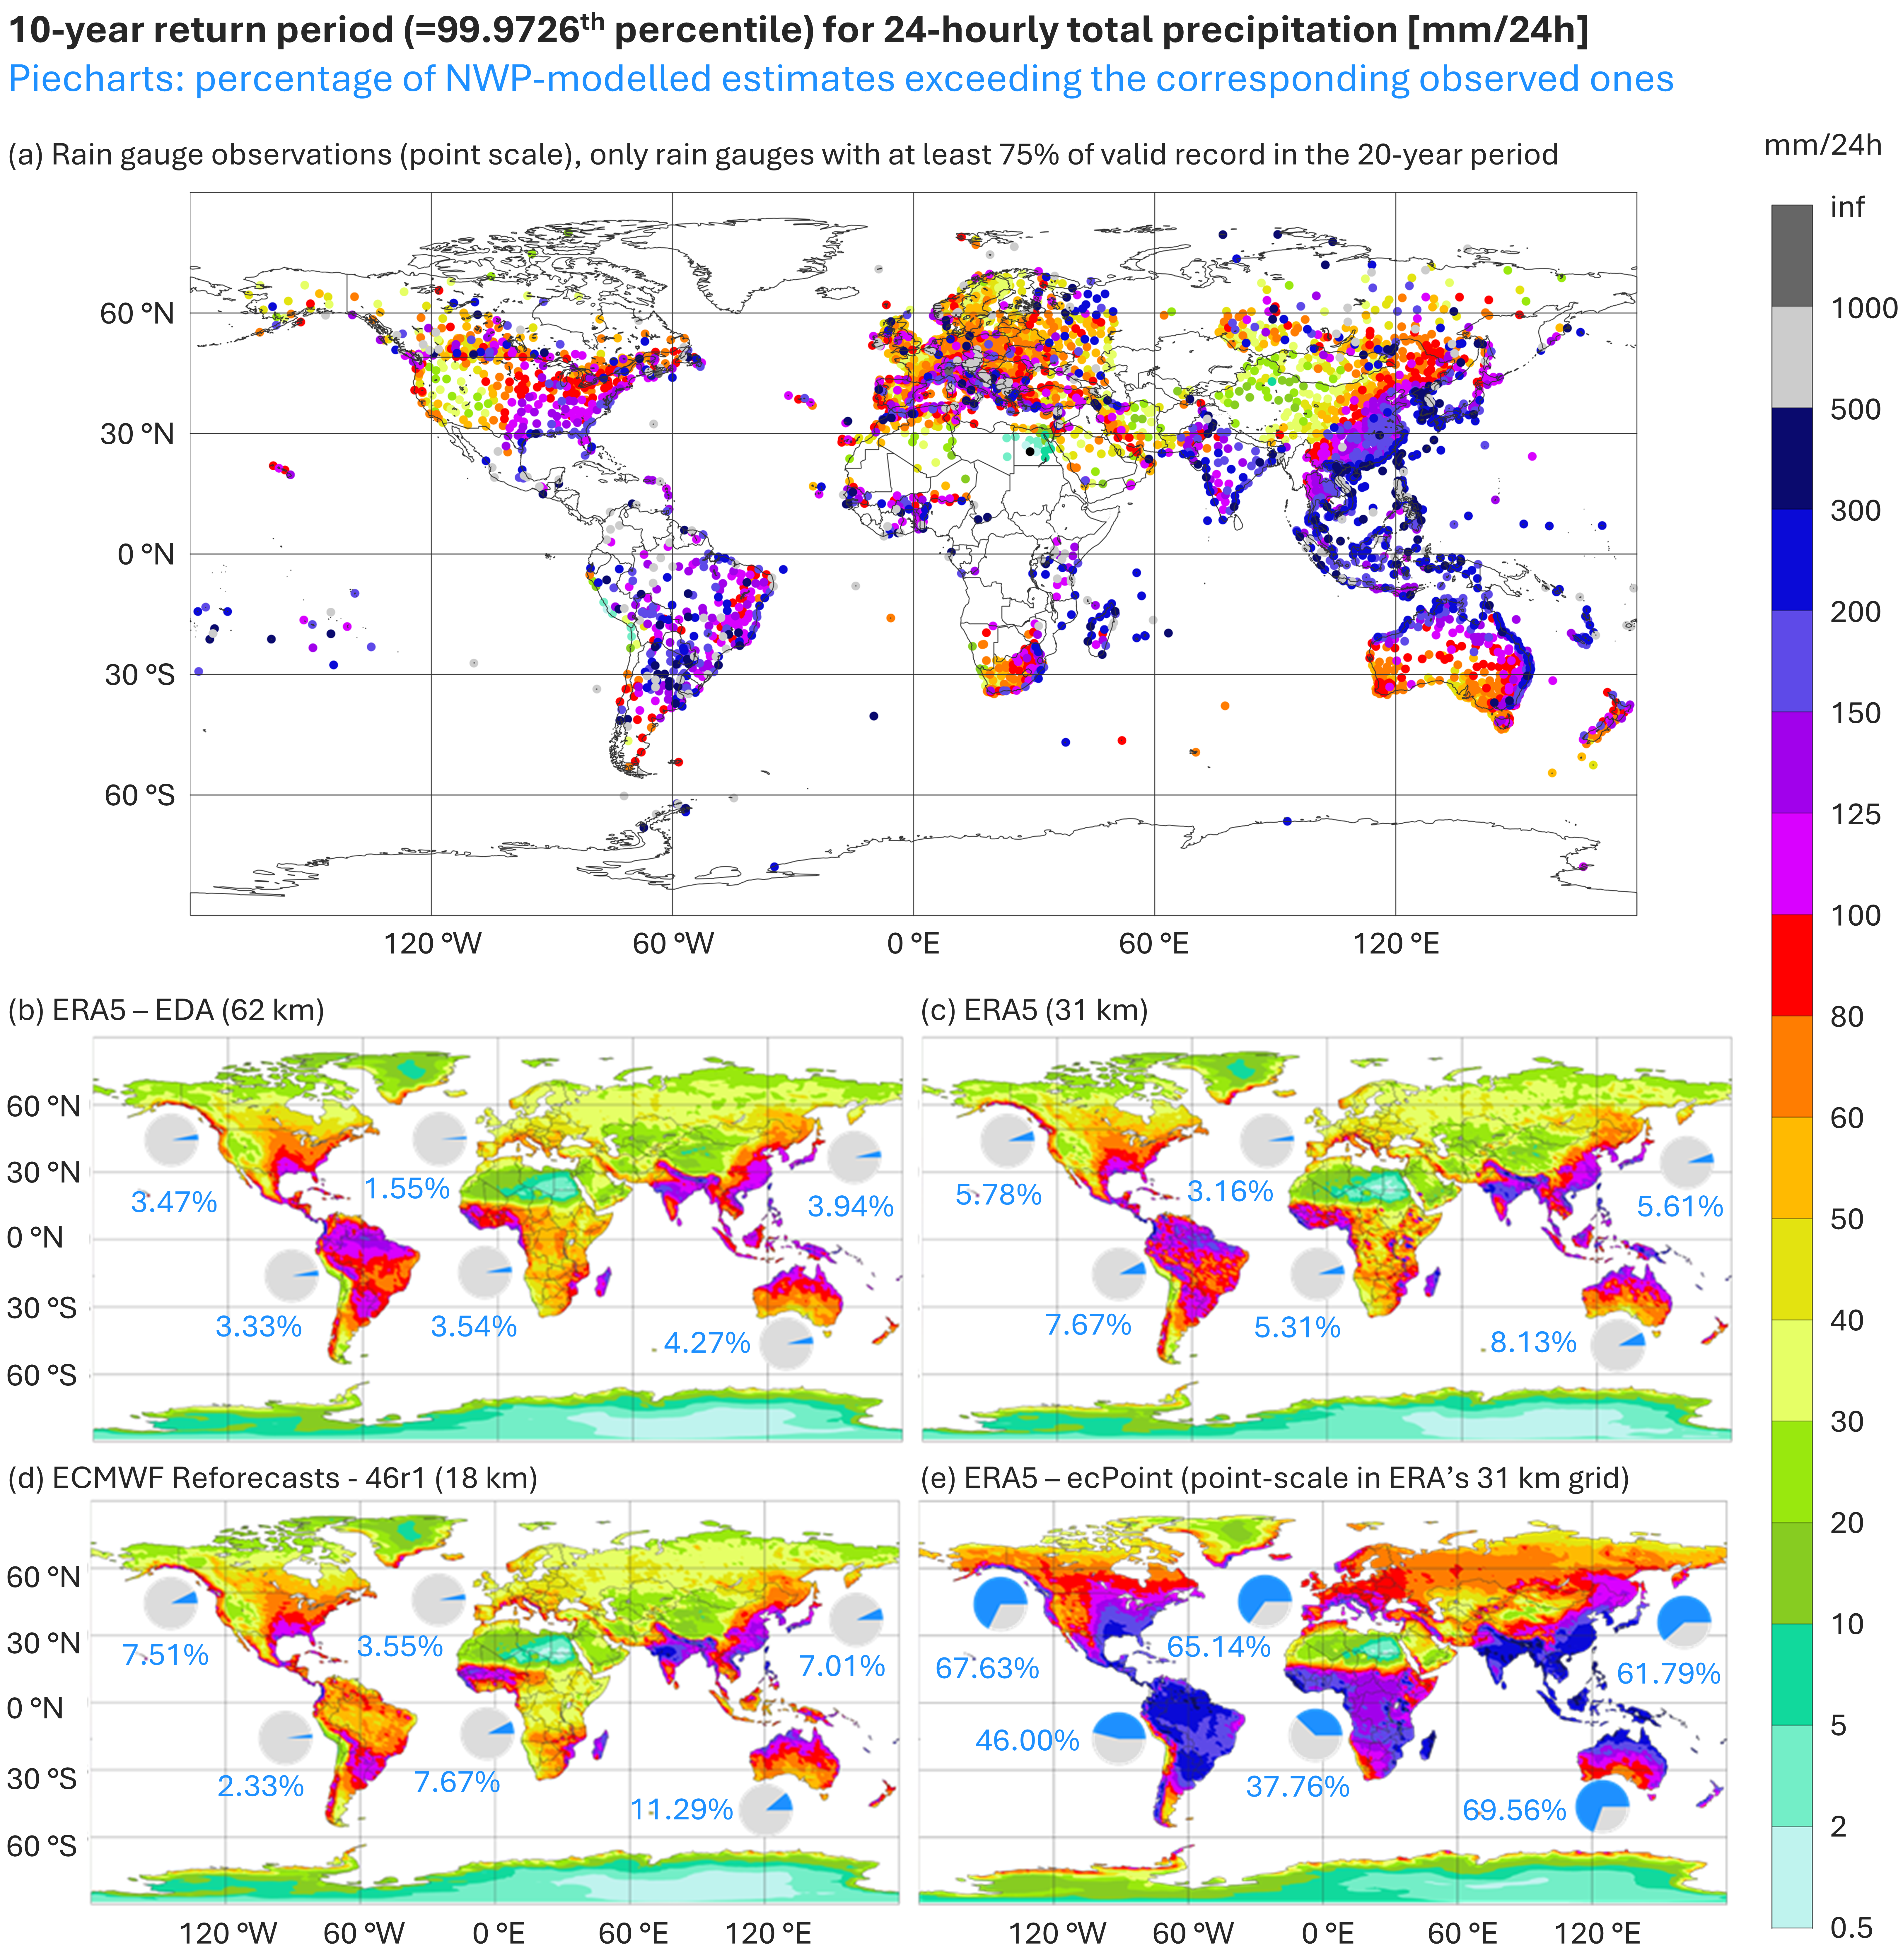
\includegraphics[width=\textwidth]{Figures/09_OBS_NWP_Rainfall_10RP.jpg}
\caption{Panel (a) displays the 10-year return period (computed from the 99.9726\textsubscript{th} percentile) for 24-hourly total precipitation from rain gauge observations, calculated over the 20-year period between 2000 and 2019, and using only rain gauges with at least 75\% of valid records. Panels (b) to (e) show the 10-year return period for NWP-modelled 24-hourly total precipitation: ERA5-EDA (62 km), ERA5 (31 km), ECMWF Reforecasts-46r1 (18 km) and ERA5-ecPoint (point-scale, provided on ERA5 grid). The pie charts represent the percentage (in \%) of modelled climatologies exceeding the observed climatologies \textcolor{teal}{over the domains defined in Figures \ref{fig:MAE_ERA5_ecPoint} to \ref{fig:MAE_Reforecasts_46r1}.}}
\label{fig:OBS_NWP_Rainfall_10RP}
\end{figure*}

The precipitation maps for the 10-year return period show that ERA5-ecPoint provides a better representation than the raw NWP models. In North America, the extremes in 24-hourly precipitation over the west coast of Alaska, Canada and North-West USA, which reach peaks up to 500 mm, are better represented in ERA5-ecPoint than in ERA5-EDA, ERA5, and reforecasts that tend not to exceed 125 mm. The peaks around the Gulf of Mexico, the USA's East Coast and the border between Canada and the USA are also better represented in ERA5-ecPoint. However, in the latter case, there seems to also be sampling-related noise in the observations. The raw NWP models better represent the extremes over the Rocky Mountains since ERA5-ecPoint overestimates them. However, the latter shows an overall closer representation of the observed ECDFs apart from the tail. ERA5-ecPoint greatly improves the precipitation peaks over Mexico and South America over the other three NWP models, apart from the Andean region and the desert on the west coast of Peru and Chile, where ERA5-ecPoint overestimates the wet tails (as shown in section \ref{results}.\ref{compare_climatologies}). It is worth noting that the ECMWF reforecasts from 46r1 halved the precipitation extremes over the Amazon compared to ERA5-EDA and ERA5. 

The extremes over Europe also verify better on ERA5-ecPoint than the three raw NWP models. The wetter climatology with peaks up to 300-500 mm around the Mediterranean catchment (including the African part), the Alps, the Atlantic coast of Spain and the UK, and the Norwegian Fiords is better captured in ERA5-ecPoint than in the three raw NWP models. The higher spatial resolution in the reforecasts helps to increase the extremes compared to both reanalyses, but they still do not exceed 100 mm in 24-hours. 

In Asia, there is a varied picture. The raw NWP models highlight the wetter climatologies of India (especially the Northeast regions), East China, Japan, Southeast Asia, and the Malay Archipelago. However, they do not reach the peaks of 300-500 mm/24h seen in the observations. ERA5-ecPoint represents such peaks. However, the peaks greater than 500 mm/24h observed in the Malay Archipelago remain underestimated, also in the post-processed ERA5. The overall overestimation in the mountainous regions of Western China has a similar flavour to the ones discussed over the Rocky Mountains in the USA: ERA5-ecPoint shows the best overall representation of the full observed ECDFs, but tends to overestimate the wet tails. In the Arabian Peninsula, all models represent the overall observed ECDF tails quite well. As discussed in section \ref{results}.\ref{compare_climatologies} for desert areas, such good representation originates from the high frequency of zero precipitation totals well estimated by all NWP models. The only exception is on the peninsula's south coast, where precipitation peaks can reach 200 mm/24h, and raw NWP models estimate a maximum peak of only up to 80 mm/24h. ERA5-ecPoint increases them up to 150 mm/24h. In Oceania, all NWP models show a good overall representation of the observed ECDFs with slight underestimations of the wet tails. The added value of ERA5-ecPoint in this region mainly provides a better representation of the precipitation peaks. There are a few observations in Africa, and nothing can be said about the model representation of precipitation extremes in the numerous ungauged areas of this continent. All NWP models represent the wet climatology of West Africa, including its Atlantic coast. However, ERA5-ecPoint best represents the observed local peaks that vary between 100 and 500 mm/24h. It is worth noting that ECMWF 46r1 reforecasts degrade the representation of the extreme precipitation around the Gulf of Guinea by producing maximum peaks only up to 80-100 mm/24h. Similarly, out of all NWP models, ERA5-ecPoint somewhat better represents the varied precipitation peaks, between 80 and 500 mm/24h, in South Africa, where raw NWP models suggest extreme precipitation might not exceed 80 mm/24h. Also, in East Africa, ERA5-ecPoint provides a more realistic representation of the extreme precipitation peaks (up to 500 mm/24h) than raw NWP models. The reforecasts considerably reduce the precipitation in this area. The wet climatology of Madagascar is well represented in all NWP models, but ecPoint can increase the wet tail of ERA5 and provide extreme precipitation totals that are closer to those observed. Finally, all NWP models seem to represent quite well the observed precipitation distribution in the Sahara, with the caveat that data coverage there is poor. In any case, good performance likely connects to the prevalence of dry weather. 

\subsubsection{Case study: Storm Vaia in Italy (28th of October 2018)}

We now examine the case of widespread (flash) flooding in Italy on the 28th of October 2018 (Figure \ref{fig:Case_Study_Italy_Flash_Floods_20181028}). This event is part of a weather system that persisted over different parts of Italy between the end of October and the beginning of November 2018. It is called Storm Vaia. In the observations (Figure \ref{fig:Case_Study_Italy_Flash_Floods_20181028}a), one can see extreme precipitation amounts between 300-400 mm/24h over Veneto (north-east), up to ~200 mm/24h over Lombardi (North) and Liguria (North-East), up to 240 mm/24h in Lazio (centre), up to 130 mm/24h in Puglia (Southwest), and up to 260 mm/24h in Calabria (Southeast). ERA5-EDA (Figure \ref{fig:Case_Study_Italy_Flash_Floods_20181028}b), ERA5 (Figure \ref{fig:Case_Study_Italy_Flash_Floods_20181028}c), and reforecasts (Figure \ref{fig:Case_Study_Italy_Flash_Floods_20181028}d) provide a good signal on which might be the wetter areas in Italy for that day, apart from the south of Italy, that does not stand out as a possible area at risk of extreme precipitation. The precipitation peaks over the Italian Peninsula increase with the increasing spatial resolution of the NWP models, but they do not reach the observed extreme precipitation totals. ERA5-EDA estimated a maximum total of ~100 mm/24h, and ERA5 pushed the estimated peaks to 150 mm/24h over Veneto. Reforecasts increased the precipitation peaks in Veneto and Lazio up to 200 mm/24h, but precipitation in Liguria, Puglia, and Calabria remains highly underestimated. ERA5-ecPoint (Figure \ref{fig:Case_Study_Italy_Flash_Floods_20181028}e) represents better the areas where the precipitation peaks were observed. In the north (Figure \ref{fig:Case_Study_Italy_Flash_Floods_20181028}f, Northern Italy), where the storm created the biggest impacts, roughly 1\% of the rainfall observations exceeded the 99th percentile of ERA5-ecPoint (red dots), indicating reliable point-scale rainfall estimates. In the rest of the peninsula (Figure \ref{fig:Case_Study_Italy_Flash_Floods_20181028}f, Central and Southern Italy), 6\% of the observations exceed the ERA5-ecPoint estimates, indicating an under-prediction of point-scale rainfall over Le Marche, Puglia, and Calabria. In this specific case, the location of the red dots along coastlines indicates underestimation primarily due to the known issue of convective cells generated over the sea not moving onto land \textcolor{teal}{\citep{Bechtold2014}}.

\begin{figure*}
\centering
\includegraphics[width=\textwidth]{Figures/10_Case_Study_Italy_Flash_Floods_20181028.jpg}
\caption{Widespread (flash) flooding in Italy on the 28th of October 2018 due to Storm Vaia. Panel (a) represents the rain gauge observations. Panels (b) to (d) show the deterministic rainfall estimates, respectively, for ERA5-EDA at 62 km (from control run), ERA at 31 km (single realisation), and ECMWF Reforecasts from 46r1 at 18 km (from control run, day 1 lead time). Panel (e) shows the probabilistic rainfall estimates from ERA5-ecPoint (99th percentile). Panel (f) shows the locations of the rain gauge observations exceeding the ERA5-ecPoint estimates at the 99th percentile. The representation is split into two geographical areas: Northern and Southern Italy, with pie charts denoting total counts for these two areas.}
\label{fig:Case_Study_Italy_Flash_Floods_20181028}
\end{figure*}


%%%%%%%%%%%%%%%%%%%%
\textcolor{magenta}{\section{Discussion}}

The results from this study show that ERA5-ecPoint provides, overall, the best representation of point-rainfall distributions out of all the NWP models tested. Specifically, ERA5-ecPoint captures better the frequency of the observed zero rainfall totals, the growth rate within the rainfall observation CDFs, and the longer wet tails. The bigger improvements are particularly evident in flat and hilly/mountainous regions. However, in very mountainous areas such as the Andes, ERA5-ecPoint underestimates the frequency of zero rainfall totals and overestimates the length of the wet tails, raising some questions about its effectiveness over very complex orography. \textcolor{teal}{This should not be surprising}, as ERA5-ecPoint is post-processed with observations primarily coming from valleys and hilly areas, although, on the other hand, verifying data comes from such sites too. \textcolor{teal}{There likely exists a complex interplay, whereby} data from non-mountainous regions is sometimes used to train for mountainous areas, despite the inclusion of a sub-grid orography variable in the ERA5-ecPoint decision tree. The growth rate of the ERA5-ecPoint rainfall estimates closely aligns with that of the observations, indicating that the post-processing system is making meaningful adjustments to the rainfall estimates. Additional observational data from regions at high altitudes are necessary to refine the corrections, particularly to increase the accuracy in representing the frequency of zero rainfall totals and to reduce the overestimation observed in the wet tail. 

Overall, the raw NWP models (i.e., ERA5-EDA, ERA5, and ECMWF Reforecasts – 46r1) consistently show an underestimation of the zero rainfall totals and the wet tails, and the growth rate of the modelled rainfall estimates is consistently bigger than that observed. This means that the raw NWP models overestimate the frequency of small rainfall totals and underestimate the frequency of extreme rainfall events, as one might expect from representivity considerations, and as has been reported previously by National Meteorological and Hydrological Services around Europe \citep{Hewson2024_3}. ERA5 (at 31 km) improves the overall representation of point-rainfall distributions compared to ERA5-EDA (at 62 km), especially in mountainous regions such as the Rocky Mountains, the Alps, and the Norwegian Fjords. However, the improvements in these regions remain modest in proportion, despite the twofold increase in spatial resolution. The ECMWF Reforecasts provide general improvements due to the increased spatial resolution (18 km) and a more up-to-date model version (46r1 rather than 41r2 of ERA5-EDA and ERA5). The observed degradations over Australasia and Africa in 46r1 (see pie charts on Figure \ref{fig:MAE_ERA5_EDA}) are counterintuitive and may be symptomatic of a physics issue that manifests in those areas. Compared to ERA5, the 46r1 improvements are focused again on mountainous areas and extend to most of Europe, the arid regions of Northern Africa, and the Arabian Peninsula. 

Focusing on extreme rainfall events, there is a general increase in the values with the increase of the raw NWP models' spatial resolution, which better agrees with the observed wetter tails. The major difference is observed between ERA5-EDA and ERA5, while the differences between the latter and the ECMWF reforecasts are less prominent. Indeed, for the rainfall in the Amazon region, Equatorial Africa, and Indonesia, the reforecasts show rainfall estimates that do not exceed 100 mm/24h. In contrast, both reanalysis, ERA5-EDA and ERA5, show rainfall estimates up to 300 mm/24h, which better represent the observed rainfall totals in the region. These results similarly contradict expectations and may indicate regional limitations in cycle 46r1 employed for the reforecast dataset.  

When focusing on extreme precipitation events, ERA5-ecPoint consistently demonstrates a superior ability to replicate observed extremes compared to raw NWP models. For example, the 10-year return period precipitation maps show that ERA5-ecPoint provides a much closer representation of observed extreme rainfall events in regions like North America, Europe, and parts of Asia. The Italian case study on Storm Vaia further underscores this finding. While raw models captured the general distribution of wetter areas, they underestimated the magnitude of precipitation peaks across multiple regions, including Veneto, Lazio, and Liguria. ERA5-ecPoint, on the other hand, was able to capture these extremes better, providing a more realistic forecast of the potential for flash floods. Some underestimation of rainfall along coastlines is highlighted due to non-moving convective cells generated over the sea that fail to generate rain over the land. Convective cell drift is something that has been explored in the ecPoint framework, but not implemented yet. Applying it should bring intrinsic improvements in the areas of triggering, via the bias correction aspect (as shown in the \citet{HewsonPillosu2021}, Norway example). 

Furthermore, ERA5-ecPoint enables one to estimate rainfall events with significantly longer return periods than those presented in this study (e.g., up to a 1000-year return period, as noted in Table 1, row 5, column 8). \citet{Hewson2024_2} have shown for 2023 Storm Daniel in Libya that applying the ecPoint post-processing technique to ERA5 can deliver usable estimates of an n-year return period rainfall from m years of data, where ${n \gg m}$. Consequently, datasets like ERA5-ecPoint offer valuable insights into the potential magnitude of extreme rainfall events, improving our preparedness for unseen events \citep{Heinrich2024, Ommer2024} or ones so infrequent that they have faded from collective memory \citep{Ludwig2023, Merz2024}.

One area where ERA5-ecPoint did not seem to provide significant benefits, and where extremes were overestimated, was in the high-altitude and relatively dry western parts of the USA, where mountain barriers can block external moisture sources. Parts of inland northern China fall into the same class. Dry boundary layers often characterise such areas. We know from experimenting with ecPoint and considering physics that low-level rainfall under-evaporation in such situations can lead to large net positive raw model rainfall biases at the grid scale, particularly in convective situations. Although ERA5-ecPoint includes a low-level humidity parameter within its decision tree, which can combat such biases, it is probably not activated in enough weather-type scenarios to be fully effective. Hence, there is some cross-contamination in the calibration from data in areas with much moister boundary layers. This could thus be a focal point for future work. While ecPoint's remote calibration approach has shown significant benefits compared to a purely local approach, as in this paper and in \cite{HewsonPillosu2021}, there can evidently be some local downsides.

\textcolor{blue}{The climatological distributions evaluated here pool observations across all months of the year without seasonal stratification, and focus exclusively on liquid precipitation as recorded by rain gauges. This design choice was deliberate: the primary objective is to assess each dataset's ability to represent the overall statistical distribution of 24-hourly rainfall accumulations across a wide range of climatic regimes, rather than to diagnose season-dependent performance. However, pooling across seasons may mask compensating biases (for instance, a model that overestimates light frontal rainfall in winter but underestimates intense convective rainfall in summer could produce an aggregate distribution that appears well calibrated despite meaningful seasonal errors). Similarly, in regions where a substantial fraction of annual precipitation falls as snow, the rain gauge observations inherently exclude that component, meaning the verification characterises only the liquid-phase subset of the precipitation climate. Decomposing the verification by season, and potentially by dominant precipitation type, would provide a more complete picture of each dataset's strengths and weaknesses across different meteorological regimes. This could represent a natural extension of this work.}

The general improvements provided by ERA5-ecPoint open up significant opportunities across various fields of environmental research that require a more accurate representation of point rainfall estimates. We advocate that such improvements would enhance both long-term strategic planning (e.g., using this dataset for climatological studies) and short-term emergency response (e.g., this dataset to create point-scale rainfall thresholds that are compatible with ecPoint rainfall medium-range forecasts to determine areas at risk of extreme localised rainfall), thereby contributing to developing more resilient societies in the face of climate change. In the realm of flood forecasting, more accurate rainfall estimates at local scales are crucial for predicting runoff and streamflow dynamics, particularly in catchments prone to flash floods. Precise point-scale rainfall data is pivotal in enhancing early warning systems, which are essential for safeguarding communities from the severe impacts of extreme rainfall and flooding. Better rainfall representation could facilitate more efficient management of reservoirs and irrigation planning in water resource management, optimising water storage and distribution for agriculture, power generation, and urban water supply systems. Furthermore, enhanced point-scale precipitation estimates are crucial for designing more resilient stormwater infrastructure and urban drainage systems, which are facing increasing pressure from the intensification of extreme rainfall events due to climate change. In the context of disaster preparedness, ERA5-ecPoint's ability to capture the full spectrum of rainfall values, including zeros and extremes, provides valuable insights into the risks posed by changing precipitation patterns.


%%%%%%%%%%%%%%%%%%%%%
\section{Conclusions}

Modern-day NWP systems and reanalysis products do not provide a good representation of 24h climatological rainfall distributions for gauged sites around the world, whilst ecPoint, in its ERA5 variant form, though not perfect everywhere, \textcolor{teal}{performs much better}.

This study provides a systematic, global verification of how well NWP models represent the distribution of point-rainfall observations. It considered point-rainfall observations over 20 years and four different modelled, gridded datasets with distinct spatial resolutions: ERA5-EDA (62 km), ERA5 (31 km), ECMWF Reforecasts for 46r1 (18 km), and ERA5-ecPoint (point-scale but provided over ERA5's grid at 31 km). Among the tested models, this study shows that ERA5-ecPoint most accurately captures both the frequency of zero rainfall totals and the wet tails of the observed point-rainfall distributions.

Since ERA5-ecPoint provides rainfall totals over a continuous global domain, the post-processed reanalysis could be used to provide seamless point-rainfall estimates, including over regions with sparse or no rain gauge observational data. \textcolor{magenta}{While increasing NWP ensemble size addresses only grid-scale forecast uncertainty and convection-permitting resolutions (~1 km) that could explicitly resolve sub-grid rainfall variability remain computationally prohibitive for global multi-decadal applications, statistical post-processing approaches such as ecPoint offer a practical and operationally viable means of bridging the scale gap between NWP grid-box averages and point-scale observations.}

However, caution is needed when generalising the verification results. While ERA5-ecPoint demonstrates strong performance in estimating point-rainfall totals overall, it is essential to note that the verification dataset contains large regions with sparse or no rain gauge observations. Furthermore, ERA5-ecPoint has shown some limitations in very complex mountainous terrains (e.g. the Andes), where the post-processed reanalysis remains short in representing the frequency of zero rainfall totals and overestimates the wet tails. Hence, this finding highlights the need for further refinement of the post-processed forecasts in these regions by incorporating, when available, more rain gauge observations in the calibration process.

The improved performance of ERA5-ecPoint over raw NWP models in representing point-scale rainfall totals, whether small or large, emphasises post-processing's critical role in addressing the inherent limitations of gridded rainfall estimates in guiding point-scale rainfall. \textcolor{teal}{The effectiveness of ecPoint, however, remains contingent} on the quality of the underlying NWP models it post-processes. Without accurate raw NWP estimates at a grid-scale, the skill demonstrated by the ERA5-ecPoint rainfall estimates would be diminished. Moving forward, the authors advocate enhancing the spatial resolution and the skill of raw NWP models alongside ongoing improvements of post-processing techniques such as ecPoint to reduce further errors in estimating the whole distribution of point-rainfall totals. Such improvements will be particularly significant as climate change intensifies the frequency and severity of extreme rainfall, making accurate and reliable point-rainfall estimates indispensable for effective mitigation and response efforts related to droughts, extreme rainfall, flooding, food security, and urban resilience.



%%%%%%%%%%%%%%%%%%%%%%%%%%%%%%%%%%%%%%%%%%%%%%%%%%%%%%%%%%%%%%%%%%%%%
% ACKNOWLEDGMENTS
%%%%%%%%%%%%%%%%%%%%%%%%%%%%%%%%%%%%%%%%%%%%%%%%%%%%%%%%%%%%%%%%%%%%%
\acknowledgments
The authors gratefully acknowledge Hans Hersbach, Paul Berrisford, and Adrian Simmons for their invaluable insights on the characteristics of ERA5 and ERA5-EDA datasets and their implications in the outcomes shown in this paper. 


%%%%%%%%%%%%%%%%%%%%%%%%%%%%%%%%%%%%%%%%%%%%%%%%%%%%%%%%%%%%%%%%%%%%%
% DATA AVAILABILITY STATEMENT
%%%%%%%%%%%%%%%%%%%%%%%%%%%%%%%%%%%%%%%%%%%%%%%%%%%%%%%%%%%%%%%%%%%%%
\datastatement
Data and/or the codes used to generate the figures that are incorporated into this manuscript will be made available upon reasonable request.


%%%%%%%%%%%%%%%%%%%%%%%%%%%%%%%%%%%%%%%%%%%%%%%%%%%%%%%%%%%%%%%%%%%%%
% REFERENCES
%%%%%%%%%%%%%%%%%%%%%%%%%%%%%%%%%%%%%%%%%%%%%%%%%%%%%%%%%%%%%%%%%%%%%
\bibliographystyle{ametsocV6}
\bibliography{references}


\end{document}